\documentclass[english,biblatex]{lni}
\usepackage{hyperref}
\usepackage[backend=biber]{biblatex}
\addbibresource{systems-engineering.bib}
\ExecuteBibliographyOptions{}
\graphicspath{{figures/}}
\DeclareGraphicsExtensions{.pdf,.jpeg,.jpg,.png}
\graphicspath{{figures/}}
\usepackage{subcaption}

\begin{document}

\title[Improving the Efficiency of Dislocality Constraints]{Improving the Efficiency of Dislocality Constraints for an Automated Software Mapping in Safety-Critical Systems}
%%% \subtitle{Untertitel / Subtitle} % if needed
\author[Robert Hilbrich \and Michael Behrisch]
{Robert Hilbrich\footnote{German Aerospace Center (DLR), Rutherfordstr. 2, 12489 Berlin,
Germany \email{robert.hilbrich@dlr.de}} \and
Michael Behrisch\footnote{German Aerospace Center (DLR), Rutherfordstr. 2, 12489 Berlin,
Germany \email{michael.behrisch@dlr.de}}}
\startpage{11} % Beginn der Seitenzählung für diesen Beitrag / Start page
%\editor{Herausgeber et al.} % Names of Editors
\booktitle{SE’18: Software Engineering-Tagung der Gesellschaft für Informatik (GI)} 
\year{2018}

\startpage{1}

\maketitle

\begin{abstract}
This is a brief overview of the paper, which should be 70 to 150 words long and
include the most relevant points. This has to be a single paragraph.
\end{abstract}


\begin{keywords}
Keyword1 \and Keyword2
\end{keywords}


\section{Introduction}

Engineering complex and safety-critical systems, such as flight control systems aboard an airplane, is still challenging and costly.
Despite recent advancements in our model-based tool suites and engineering methods, the design of these systems still bears risk and uncertainties with regard to its outcome.
The formalization and automation of crucial engineering tasks appears to be a promising approach to tackle these challenges~\cite{Chapman2007}.
Systems in these areas are engineered to implement a complex interplay between mechanical elements, electronic components, as well as (embedded) software.
Therefore, their design has to mirror this interplay and requires the development of a hardware and software architecture.

In practice, these architectures can often be developed independent of each other, but their integration in the final system requires a \emph{link} between the software components and their hardware resources.     
This \emph{link} is referred to as a \emph{deployment} of the software components.
Constructing a deployment requires the systems engineer to \emph{map} software components to resources and to \emph{schedule} the access to shared resources.
Therefore, mapping refers to a \emph{spatial allocation}, while scheduling refers to a \emph{temporal allocation} of software components.

The construction of a deployment is an engineering task, which not only affects the fulfillment of functional requirements by providing the necessary, but also affects the satisfaction of non-functional requirements, such as safety and reliability.
Redundancy and fault tolerance can only be achieved, if critical software components are deployed accordingly.

The construction of a deployment is a very elaborate task with zero tolerance for errors as they may jeopardize the correctness of the system.
At the same time, it requires a detailed understanding of the requirements of all software components and the capabilities of all hardware resources in the system.
Due to the sensitivity and complexity of this task, its formalization and automation is a valuable research goal.

\section{Automated Construction of Deployments}

In order to achieve an automated construction of a deployment and to argue its correctness, a formalization of the mapping problem is required.
For smaller mapping problems, this has been successfully achieved based on Linear Integer Programming~\cite{Damm2006, Kugele2009}, SMT-based solvers~\cite{Voss2013} or evolutionary algorithms~\cite{White2011}.
However, these approaches reach their limits when larger, real-world mapping problems with limited gradient information to guide a search process are considered.

The authors instead chose to transform a mapping problem into a semantically equivalent \emph{Constraint Satisfaction Problem (CSP)}~\cite{Apt2003,Dechter2003} and solve this CSP with \emph{Constraint Programming} techniques~\cite{Rossi2006,Prudhomme2016}.
The advantages of using Constraint Programming in comparison to other techniques lie in the availability of powerful modeling elements, such as an \textsc{allDifferent} constraint, and the ease with which custom search heuristics can be implemented.

\subsection{Constraint Satisfaction Problems}
Constraint Programming refers to a set of techniques in artificial intelligence and operations research.
These techniques assist in finding solutions for problems based on variables, which are affected by constraints.
Each constraint defines valid or invalid solutions for a subset of these variables.
In this paper, a subclass of constraint satisfaction problems is used to express mapping problems:  \emph{finite domain integer constraint satisfaction problems} in which each variable has a finite integer domain.
Solutions for this problem class can be obtained by applying a combination of \emph{search} techniques -- including backtracking -- and constraint \emph{propagation} techniques for value elimination.

To illustrate the modeling approach of Constraint Satisfaction Problems, consider the well-known \emph{Map Coloring} problem as an example.
This problem asks, whether it is possible to color a map with only four colors in such a way, that neighboring countries have different colors.
It can be formulated as a CSP by assigning an integer variable $x_i$ for each country with the index $i$.
The domain of each variable corresponds to the four colors: $D_{x_i}=\{0,1,2,3\}$.
In order to model the restrictions of this problem, a constraint is added for each pair of adjacent countries.
If country $x_i$ is adjacent to country $x_j$, then $x_i \neq x_j$ is required.
The search algorithm is now responsible to select a variable and test a value of its domain.
Assuming a simple ``first variable, first value'' strategy, the variable $x_0$ would be chosen and set to the value $0$ as a test.
This would be \emph{propagated} to all variables which are directly linked to $x_0$ by a constraint, so that the value $0$ gets removed from their domains.
This removal may lead to other value removals in indirectly linked variables and is processed until a fix point is reached.
If a contradiction is encountered or the domain of a variable becomes empty, \emph{backtracking} is initiated, so that the next value of the variable $x_0$ is tested.
Otherwise, the search algorithm continues with the next uninstantiated variable.

This example also shows, that the propagation of the \textsc{NotEqual} constraint is \emph{weak}, because it affects only two variables and invalidates only 4 out of the 16 possible value combinations between two variables.

\subsection{Toolsuite ASSIST}

As a proof of concept for the ongoing research toward an automated construction of deployments based on Constraint Satisfaction Problems, the toolsuite \emph{Architecture Synthesis for Safety-Critical Systems (ASSIST)}~\cite{ASSIST} was developed by the authors.
It is publicly available under the Eclipse Public License 2.0 and uses the constraint solver \emph{Choco 4}~\cite{Prudhomme2016} internally.

\begin{figure}[htbp]
\centering
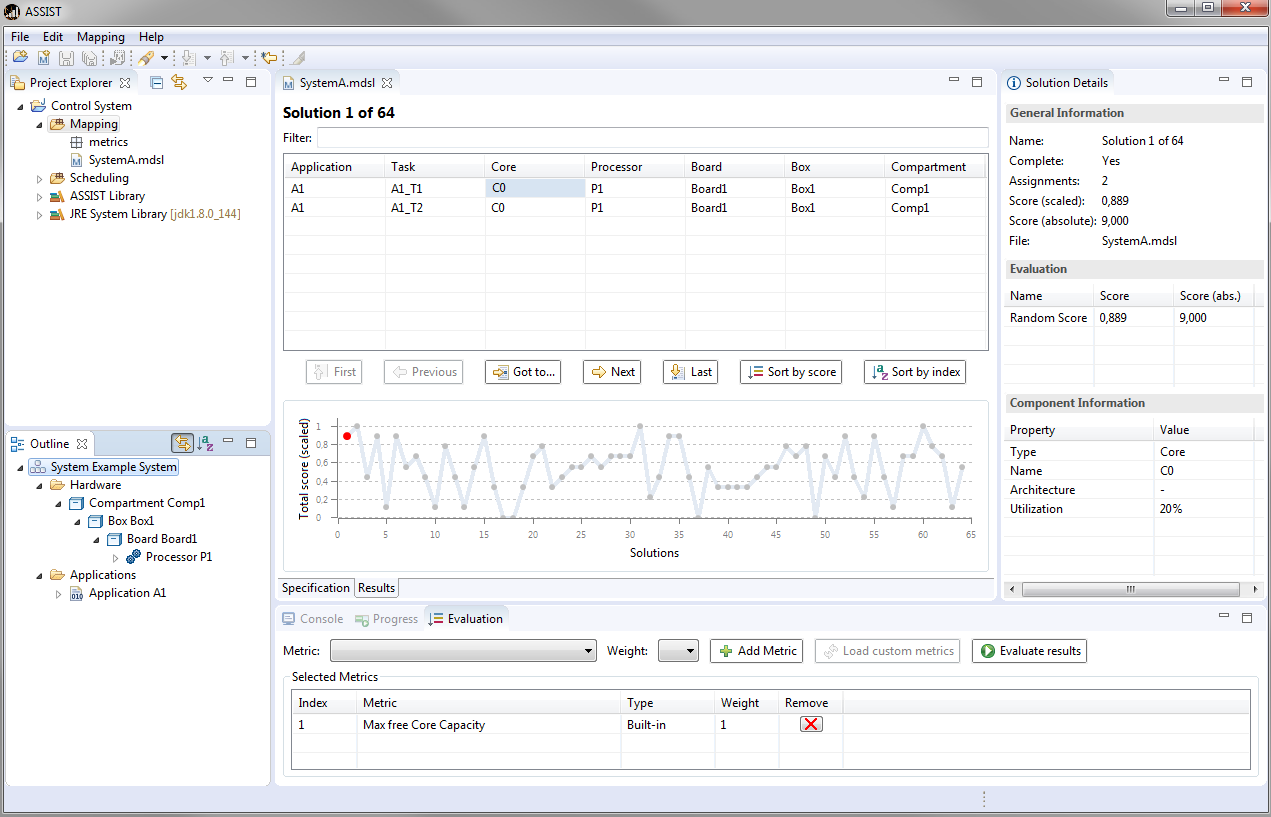
\includegraphics[width=\textwidth]{assist-screenshot}
\caption{Screenshot of ASSIST with a specification for a control system}
\label{tool}
\end{figure}

ASSIST (see Figure~\ref{tool}) allows a systems engineer to automatically construct and optimize mappings and schedules based on textual specifications of the

\begin{itemize}
\item software components and hardware resources,
\item \textit{dislocality}, \textit{dissimilarity} and \textit{colocality} requirements,
\item optimization goals.
\end{itemize}

The textual specifications in ASSIST conform to a domain-specific language which allows to hide the intricacies of a formal specification.
Using a domain-specific language is expedient to enable systems engineers without a formal education in computer science to precisely specify a deployment problem.

\section{Ensuring Fault Tolerance by Requiring Dislocality}

In order to achieve fault tolerance and reliability, it is essential to support ``significant differences'' in the choice of resources to which critical software components are deployed to.
For instance, a simple redundancy requirement between two software components, may force the systems engineer to allocate these software components to different processing boards in different locations aboard an airplane.
Furthermore, systematic errors and undetected design flaws in hardware components may be addressed by choosing dissimilar hardware resources, for example processors or memory blocks from different vendors.

Due to the importance of choosing  ``different'' resources for fault tolerance and reliability in safety-critical systems, engineering tools for an automated construction of deployments need to be able to fully support these choices.
ASSIST supports the engineer by offering \emph{dislocality} and \emph{dissimilarity} requirements as part of the domain specific language.
They can be used to enforce ``differences'' for the choice of resources for the mapping of software components.
Finding an \emph{efficient} formulation to express the semantics of each requirement as a Constraint Satisfaction Problem is challenging, but also essential in order to provide an effective toolsuite for the engineering of safety-critical systems.

In order to illustrate the challenges and to present specific modeling improvements, the \emph{dislocality} requirement is used as an central example in this paper.
Please note, that the concepts developed for \emph{dislocality} requirements can also be reused for \emph{dissimilarity} requirements.

The semantics of a dislocality requirement can be illustrated with the following deployment problem (see Figure~\ref{example}).
In the example system, there are three \emph{applications} consisting of one or more \emph{tasks}.
Each task has to be mapped to exactly one of the \emph{processors} in the system.
It is assumed, that the processor contains multiple cores, so that multiple tasks can be mapped to a single processor.
However, in order to ensure fault tolerance, a \emph{dislocality} requirement is added for all applications.
This means, that the applications must not share a processor, so that a faulty processor affects only one application.

\begin{figure}
\centering
\subcaptionbox{Simple Case}{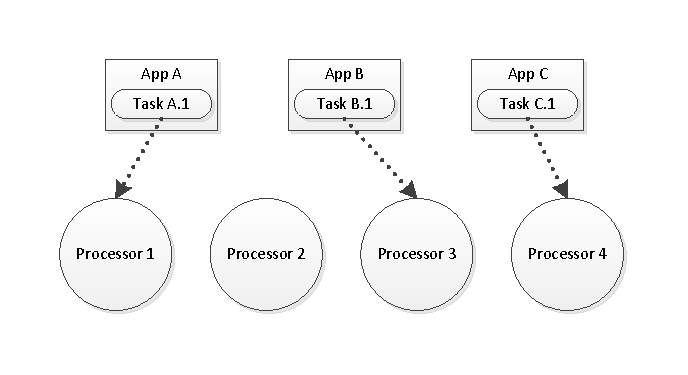
\includegraphics[width=0.47\textwidth]{application-mapping-simple}}%
\hfill
\subcaptionbox{Complex Case}{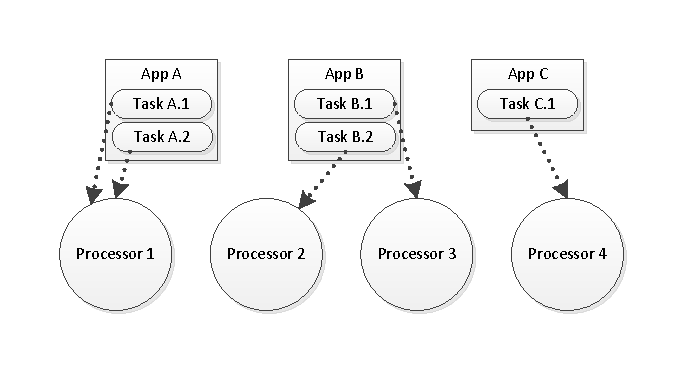
\includegraphics[width=0.47\textwidth]{application-mapping-complex}}%
\caption{An Example Deployment Problem - Mapping Tasks to Processors}
\label{example}
\end{figure}

Expressing the basic deployment problem with constraints is straight forward.
Each task $i$ in the system is represented by an integer variable $X_i \in \{0, 1, \dots, n-1\}$. The domain of each variable $X_i$ corresponds to the indices of the $n$ processors in the system.
This formulation is still missing the constraints for the dislocality requirements.

In the simple case, if all applications consist of only one task, this can be achieved with a single \texttt{allDifferent} constraint (see~\cite{GCCAT2014}) over all variables $X_i$.
This situation is depicted in Figure~\ref{example}~(a).
Fortunately, Choco 4 already contains an implementation for an \texttt{allDifferent} constraint based on the algorithm of Régin~\cite{Regin1994}.

However, in reality, applications usually consist of more than just one task and tasks of the same application \emph{can} typically share the same processor.
This situation is more complex and depicted in Figure~\ref{example}~(b).
Unfortunately, in this case, the previous approach of applying a single \texttt{allDifferent} constraint over all variables $X_i$ can no longer be used.
It would prevent solutions in which a processor is shared by multiple tasks of the same application.
The existing \texttt{allDifferent} constraint only ensures, that values for a list of variables are different.
However, the complex case requires an advanced \texttt{allDifferent} constraint operating with a list of a list of variables and ensuring that the combined values for each list of variables are different.
Unfortunately, such a constraint is neither part of the Global Constraint Catalog~\cite{GCCAT2014} nor available in Choco 4.

\section{Modeling Complex Dislocality Requirements}

This section introduces three alternative implementations for the semantics of an advanced \texttt{allDifferent} constraint.
Their performance and impact on resolution time will be analyzed and compared to each other in the next section.

However, before continuing with the description of possible implementations, the semantics of an advanced \texttt{allDifferent} constraint should be described more precisely.
The example system in Figure~\ref{example}~(b) consists of the applications $A$, $B$ and $C$.
Each of these applications contains one or more tasks, for example $A = \{A_1, A_2\}$, $B = \{B_1, B_2\}$ and $C = \{C_1\}$.
An advanced \texttt{allDifferent} for all applications would be operating over a list of a list of variables:
$$\textrm{\texttt{allDifferent}}\left\{\{A_1, A_2\}, \{B_1, B_2\}, \{C_1\}\right\}$$
Assuming that $A^\star$ combines the values for each task in application $A$:
$$A^\star \in \mathcal{P}(\mathbb{N}) = A_1\cup A_2$$
and $B^\star$ and $C^\star$ do the same for the applications $B$ and $C$, then the advanced \texttt{allDifferent} constraint would ensure, that the sets $A^\star$, $B^\star$ and $C^\star$ are pairwise disjunct.

\subsection*{Element-wise Approach}

One option to implement the advanced \texttt{allDifferent} constraint semantic is to apply the already existing \texttt{allDifferent} constraint for every subset $s$ with
$$s = \{a,b,c \, \vert \, a \in A,  b \in B, c \in C\}$$
For systems with a large amount of applications and several tasks within each application, the amount of constraints, that will be added to the constraint solver by this approach, may significantly affect the resolution time.
However, this approach can be realized with the tools already available in Choco 4 and does not require any additional implementation of custom propagators and constraints.

\subsection*{Instantiation-only Approach}

In order to address the drawbacks of the first approach, another option is to implement a custom constraint and propagator for Choco 4 that is able to operate on a list of a list of variables.
The propagator only reacts on instantiation events for any of the variables.
If an instantiation is detected, then the value of the instantiated variable will be removed from the values of all variables in all the other lists.
This approach has the advantage, that only one constraint needs to be added to the constraint solver for each dislocality requirement.
However, this instantiation-only approach leads to a weak propagation as it only removes values, when one of the variables is instantiated.
Therefore, this approach relies on the application of clever search strategies in order to be efficient.

\subsection*{Combined Values-Union and Instantiation-Only Approach}



\section{Experiments}

\begin{itemize}
\item Synthetic example generator 
\item 10/20 Examples were generated with a parameter domain ...
\item Search with the same strategies DomWD, minValueFirst
\item iMac 5k, 64 GB RAM, Choco 4.0.6
\end{itemize}

\section{Results}

\begin{itemize}
\item Show results for var count, constraint count
\item Show results for resolution time
\item Show results for backtracks and fails
\end{itemize}

\section{Conclusions}

I am a summary - what shall i put here?

\printbibliography[heading=bibintoc]

\end{document}

%%% Local Variables: 
%%% mode: latex
%%% TeX-master: "paper"
%%% ispell-check-comments: exclusive
%%% ispell-local-dictionary: "english"
%%% End:
